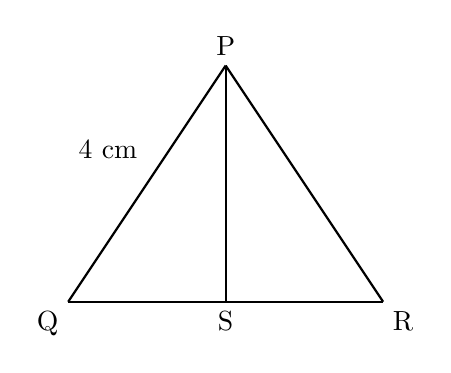
\begin{tikzpicture}

    % Define the coordinates for triangle PQR
    \coordinate (Q) at (0, 0);       % Bottom left vertex
    \coordinate (R) at (4, 0);       % Bottom right vertex
    \coordinate (P) at (2, 3);       % Top vertex
    \coordinate (S) at (2, 0);       % Point S on QR (foot of altitude)
    
    % Draw the triangle sides
    \draw[thick] (P) -- (Q);         % Side PQ
    \draw[thick] (Q) -- (R);         % Side QR
    \draw[thick] (R) -- (P);         % Side PR
    
    % Draw the altitude PS from P to QR
    \draw[thick] (P) -- (S);         % Altitude PS
    
    % Label point P
    \node[above] at (P) {P};
    
    % Label point Q
    \node[below left] at (Q) {Q};
    
    % Label point R
    \node[below right] at (R) {R};
    
    % Label point S
    \node[below] at (S) {S};
    
    % Label the measurement 4 cm on side PQ
    \node[above left] at (1, 1.7) {4 cm};
    
    \end{tikzpicture}